%! Author = danielmendes
%! Date = 13.02.25

\chapter{Replikation}\label{ch:replikation}
In diesem Kapitel befassen wir uns mit dem Thema Replikation.
Replikation ist die Grundlage für den Aufbau großer, leistungsstarker Anwendungen auf der Basis von MySQL.
Es verfolgt dabei die sogenannten "Scale-Out"-Architektur, bei der mehrere Storage-Knoten parallelisiert arbeiten und nach außen wie ein einziges Gesamtsystem (\cite{scale_out_eigenschaften}).
Dadurch ist die Skalierbarkeit nahezu unbegrenzt durch das einfache Hinzufügen weiterer Speicherknoten und nicht wie bei Scale-Up durch die Systemgrenzen eines einzelnen Geräts limitiert.
Es trägt allerdings auch Nachteile mit sich, zu denen wir u.a.\ auch später in diesem Abschnitt kommen.
In schon in den vorherigen Kapiteln gehen wir zuerst auf die Grundlagen ein, dann betrachten wir die Konfiguration, die die Basis für die Benchmarks bilden und abschließend analysieren wir die Ergebnisse.

\section{Grundlagen}\label{sec:replication-grundlagen}
Replikation ermöglicht die Konfiguration eines oder mehrere Server als Replicas eines anderen Servers (Master).
Neben der Begrifflichkeit Master-Replika, sind auch die Varianten Primary-Secondary, als auch Master-Slave üblich.
Das grundlegende Problem, das die Replikation löst, besteht darin, die Daten eines Servers mit denen eines anderen synchron zu halten.
Es können sich mehrere Replicas mit einem einzigen Master verbinden und mit diesem synchron bleiben.
Master und Replicas können in vielen verschiedenen Konfigurationen angeordnet werden.
Neben der klassischen Master-Replica-Variante können Replicas selbst als Master für weitere Replicas dienen.
Zudem ist auch eine Master-Master-Kombination möglich.
Das Prinzip der Replikation ist nicht nur für eine höhere Effizienz vorteilhaft, sondern auch für hohe Verfügbarkeit, Skalierbarkeit und Datenanalysen im Data Warehousing, aber sollte keine richtigen Backups ersetzten.
Effizienzvorteile gibt es insbesondere durch die Lastverteilung, die Leseanfragen auf mehrere Server verteilt werden, was besonders für leselastige Anwendungen vorteilhaft ist.
Außerdem kann man das Ganze mit Methoden wie Round-Robin-DNS oder Loadbalancer optimieren.

Im folgenden Abschnitt erklären wir die Funktionsweise der Replikation und betrachten dabei den einfachen Fall mit einem Master und einem oder mehreren Replicas.
Unmittelbar bevor jede Transaktion, die Daten aktualisiert, auf dem Master abgeschlossen wird, zeichnet der Master die Änderungen in seinem Binärlog (engl.\ binary log) auf.
MySQL schreibt Transaktionen seriell im Binary-Log und teilt nach dem Schreiben der Ereignisse den Storage Engines mit, die Transaktionen zu committen.
Zu diesen Änderungen können beispielsweise neu deklarierte Tabellen oder Trigger sowie Einfügeoperationen in bestehende Tabellen gehören.
Im nächsten Schritt muss die Replica die Veränderungen auf dem Masters mitbekommen.
Dazu wird ein Worker-Thread gestartet, der als I/O-Slave-Thread bezeichnet wird, und eine Client-Verbindung zum Master geöffnet.
Anschließend wird ein spezieller Prozess (binlog dump process) gestartet, der die Ereignisse aus dem Binary-Log des Masters liest.
Nach dem Verarbeiten schreibt der Thread die Werte auf seine eigene Festplatte, in das sogenannte Relay-Log.
Wenn er alle Ereignisse auf dem Log verarbeitet hat, geht er in einen passiven Zustand und wartet auf Aktualisierungen.
Den letzten Teil des Prozesses übernimmt der SQL-Slave-Thread.
Er liest und spielt Ereignisse aus dem Relay-Log ab und aktualisiert so die Daten des Replicas, sodass sie mit denen des Masters übereinstimmen.
Wenn dieser Thread eine etwa gleich schnelle Verarbeitung wie der I/O-Thread, dann bleibt das Relay-Log normalerweise im Cache des Betriebssystems, sodass Relay-Logs nur sehr geringe Overhead-Kosten haben.
Die Ereignisse, die der SQL-Thread ausführt, können optional zusätzlich in das eigene Binary-Log des Replicas geschrieben werden.

\begin{figure}[!ht]
  \centering
  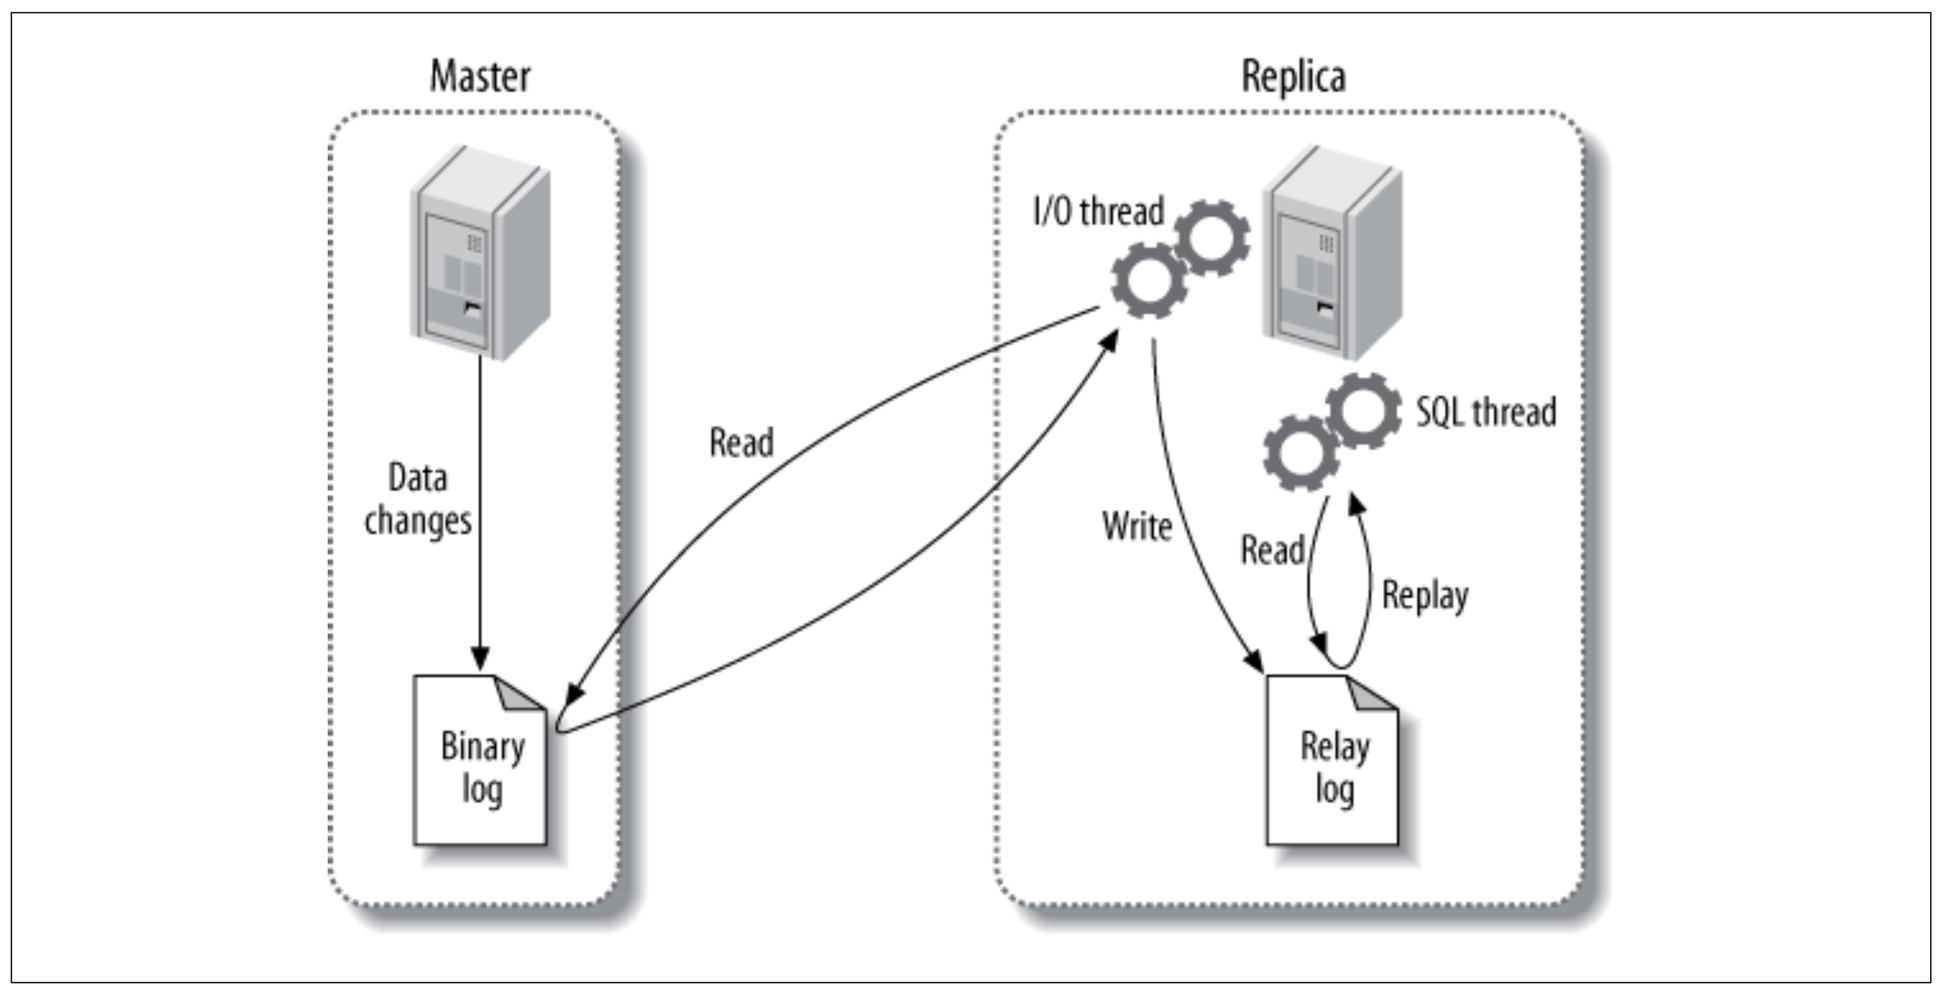
\includegraphics[width=.8\textwidth]{PNGs/Textbook/Master_Replica}
  \caption[Master - Replica - Grafik]{Darstellung der unterschiedlichen Threads}
  \label{fig:master-replica}
\end{figure}

Die Abbildung \ref{fig:master-replica} zeigt nur die beiden Replikations-Threads, die auf dem Replica laufen.
Zusätzlich gibt es jedoch einen weiteren Thread auf dem Master, da die vom Replica zum Master geöffnete Verbindung einen Thread auf dem Master startet, ähnlich wie jede andere Verbindung zu einem MySQL-Server.

Diese Replikationsarchitektur entkoppelt die Prozesse des Abrufens und Abspielens von Ereignissen auf dem Replica.
Dadurch können die beiden Threads asynchron arbeiten, sodass der I/O-Thread unabhängig vom SQL-Thread agieren kann.
Dies hat jedoch zur Folge, dass Änderungen, die parallel in verschiedenen Threads auf dem Master ausgeführt werden könnten, auf dem Replica nicht parallelisiert werden können, da sie in einem einzelnen Thread ausgeführt werden.
Generell gibt es keine Garantie für die Latenz auf der Replica und große Abfragen können dazu führen, dass die Replica Sekunden, Minuten oder sogar Stunden hinter dem Master zurückbleibt.
Der Flaschenhals (engl.\ bottleneck) des gesamten Systems stellt die Anzahl der Schreibvorgänge dar, die der langsamste Thread ausführen kann.

Die Replikation fügt dem Master nur wenig Overhead hinzu.
Das binäre Logging, das für ordnungsgemäße Backups und Point-in-Time-Recovery erforderlich ist, kann jedoch einen erheblichen Overhead verursachen.
Abgesehen davon verursacht jede angeschlossene Replica nur geringe Last (hauptsächlich Netzwerk-I/O) auf dem Master.
Das Anbinden vieler Replicas an einen Master führt einfach dazu, dass die Schreibvorgänge mehrfach ausgeführt werden, jeweils einmal auf jeder Replika.
Trotzdem sollte man nicht zu leichtfertig mit der Anzahl an Replicas übertrieben, da dadurch im Wesentlichen viele Daten unnötig dupliziert werden.
Bei sehr hoher Arbeitslast (z.B. 5.000 Transaktionen pro Sekunde) und vielen Replicas kann der Overhead durch das Aktivieren aller Replica-Threads jedoch erheblich werden.
Replikation eignet sich gut zum Skalieren von Lesevorgängen.

Die Replikation von MySQL ist größtenteils abwärtskompatibel, d.h.\ dass ein neuerer Server in der Regel problemlos als Replika eines älteren Servers fungieren kann.
Andersherum kann es aber zu Fehler kommen, da möglicherweise neue Funktionen oder die SQL-Syntax des neueren Servers nicht verstanden werden kann.
In unserem Beispiel verwenden wir ohnehin nur eine MySQL-Version (siehe \ref{sec:replication-durchfuhrung}).

Es gibt zwei verschiedene Arten der Replikation, die von MySQL unterstützt werden: die anweisungsbasierte (engl.\ statement-based) und die zeilenbasierte (engl.\ row-based) Replikation.
Die anweisungsbasierte Replikation wird seit MySQL 5.0 und älter unterstützt und funktioniert, indem die Abfrage, die die Daten auf dem Master geändert hat, protokolliert wird.
Wenn eine Replica das Ereignis aus dem Relay-Log liest und ausführt, wird die tatsächliche SQL-Abfrage erneut ausgeführt, die der Master ausgeführt hat.
Der offensichtlichste Vorteil davon ist, dass sie relativ einfach zu implementieren und das Protokollieren und Wiederholen von den Anweisungen sollte die Replica logischerweise mit dem Master synchron halten.
Außerdem sind die Binary-Log-Ereignisse in der Regel recht kompakt sind und verbrauchen nicht viel Bandbreite.
In der Praxis gibt es jedoch Änderungen auf dem Master, die von Faktoren abhängen, die über den reinen Abfragetext hinausgehen.
Beispielsweise werden Anweisungen zu leicht oder sogar deutlich unterschiedlichen Zeiten auf dem Master und dem Replica ausgeführt.
Deshalb muss der Binary Log nicht nur der Abfragetext enthalten, sondern auch Metadaten wie den aktuellen Zeitstempel.
Es gibt einige Anweisungen, die MySQL nicht korrekt replizieren kann, z.B. Abfragen, die die Funktion CURRENT\_USER() verwenden und gespeicherte Routinen und Trigger sind ebenfalls problematisch bei dieser Art der Replikation.

Die zeilenbasierte Replikation speichert die tatsächlichen Datenänderungen im Binary-Log.
Ein großer Vorteil, der daraus folgt, ist es, dass MySQL jede Anweisung korrekt replizieren kann.
Zudem können einige Änderungen mithilfe der zeilenbasierte Replikation effizienter sein, da die Replica die Abfragen, die die Zeilen auf dem Master geändert haben, nicht erneut ausführen muss.
Dies ist beispielsweise der Fall, wenn eine Abfrage viele Zeilen in der Quelltabelle scannt, jedoch nur zu drei Zeilen in der Zieltabelle ausführt.
Bei der anweisungsbasierten Replikation müsste eine Replica die Anweisung erneut ausführen, nur um ein paar Zeilen zu erstellen und bei der Zeilenbasierte ist dies effizient und trivial.
Andererseits ist das folgende Ereignis deutlich günstiger mit statement-basierter Replikation zu replizieren:

\vspace{-5pt}
\begin{lstlisting}[language=SQL,caption=Update-Befehl auf dem Master,label={lst:repl_update_command}]
UPDATE master_table SET col1 = 0;
\end{lstlisting}
\vspace{-5pt}

Die Verwendung von zeilenbasierte Replikation für diese Abfrage wäre sehr teuer, da jede Zeile geändert wird und damit auch ins Binary-Log geschrieben müsste, was das Binary-Log-Ereignis extrem groß machen würde.
Dies würde sowohl beim Protokollieren als auch bei der Replikation zu einer höheren Last auf dem Master führen.
Die Durchführung einer Point-in-Time-Wiederherstellung ist mit einem Binary-Log im row-based Format schwieriger, aber nicht unmöglich.

Insgesamt ist die anweisungsbasierte Replikation besser geeignet, wenn das Schema auf dem Master und dem Replikat unterschiedlich ist, und kann in Szenarien eingesetzt werden, in denen Tabellen unterschiedliche, aber kompatible Datentypen, verschiedene Spaltenreihenfolgen usw.\ aufweisen.
Außerdem vereinfacht es das Durchführen von Schema-Änderungen auf einem Replica, das später als Master verwendet werden soll, um möglicherweise die Ausfallzeit zu reduzieren.
Die zeilenbasierte Replikation kann jedoch einige Operationen bei Schema-Änderungen auf einem Replica nicht handhaben.
Dafür aber funktioniert sie zuverlässig mit allen SQL-Konstrukten und es gibt weniger Fälle, in denen es zu Problemen kommt.
Auch stoppt sie bei Fehlern, z.B.\ wenn eine erwartete Zeile auf dem Replikat fehlt, was jedoch auch als Vorteil betrachtet werden kann, da es auf Inkonsistenzen hinweist.
Bei der anweisungsbasierte Replikation führt ein Update auf dem Master zu keinem Fehler, wenn die Zeile auf dem Replica fehlt.
Die zeilenbasierte Replikation erkennt diesen Fehler und stoppt die Replikation, was eine sofortige Überprüfung ermöglicht.
Bei der anweisungsbasierten Replikation erfolgen alle Änderungen über einen bekannten Mechanismus (SQL-Anweisungen), was die Fehlersuche und das Verständnis von Problemen erleichtert, aber es erfordert auch mehr Sperren (Locks).
Genau andersherum sieht es bei der Zeilenbasierte aus, da dort Nachvollziehbarkeit von Änderungen ohne die Speicherung der ursprünglichen SQL-Anweisung erschwert wird, aber dafür gibt es reduziertes Locking.
Die zeilenbasierte Replikation hat auch Vorteile bei der Datenwiederherstellung, da in einigen Fällen auch alte Daten gespeichert werden, was die Wiederherstellung erleichtert.
Auch benötigt sie oft weniger CPU-intensiv, da keine komplexe SQL-Parsing- und Ausführungslogik erforderlich ist und es gibt auch Probleme bei der mehrstufiger Replikation.
Denn wenn eine Anweisung mit @@binlog\_format = STATEMENT auf dem Master ausgeführt wird, dann wird sie dort als Statement protokolliert.
Die nachgelagerte Replicas (Second-Level-Replicas) können diese jedoch als row-basiert weiterleiten, was zu Inkonsistenzen bei der Protokollierung führt.

Da kein Format in jeder Situation perfekt ist, kann MySQL dynamisch zwischen statement-basierter und row-basierter Replikation wechseln
Standardmäßig wird die statement-basierte Replikation verwendet, aber wenn MySQL ein Ereignis erkennt, das nicht korrekt als Statement repliziert werden kann, wechselt es automatisch zur row-basierten Replikation
Sie können das Format auch manuell steuern, indem Sie die Session-Variable binlog\_format setzen

\section{Durchführung}\label{sec:replication-durchfuhrung}

Für die Durchführung nutzen wir wieder die Kundentabelle (\ref{lst:create_table_kunde}) und die Bestelltabelle (\ref{lst:create_table_bestellung}), die wir schon aus dem Beispiel aus Kapitel \ref{sec:projektaufbau-mit-beispiel} kennen.
Die einzige Anpassung, die wir vornehmen müssen, sind die unterschiedlichen Werte \texttt{STATEMENT}, \texttt{ROW} und \texttt{MIXED}, die die Variable \texttt{binlog\_format} annehmen kann.

\vspace{-5pt}
\begin{lstlisting}[language=SQL,caption=Unterschiedliche Formatimplementationen,label={lst:repl_change_format}]
SET SESSION binlog_format = 'STATEMENT'
SET SESSION binlog_format = 'ROW'
SET SESSION binlog_format = 'MIXED'
\end{lstlisting}
\vspace{-5pt}

Damit können wir die Performanceunterschiede zwischen den einzelnen Arten, insbesondere für die Einfügeoperationen, vergleichen.
Wie wir sehen, sind die Veränderungen an den Lua-Skripten damit minimal, aber der eigentliche Aufwand entsteht bei der Einrichtung der Replikation auf dem lokalen Rechner und in einem Workflow.

Für die Benchmarks betrachten wir das einfachste Szenario der Replikation, bestehend aus einem Master und einer beliebigen Anzahl an Replicas.
Zunächst müssen wir dazu den Master und die Replikationsknoten dazu konfigurieren und anschließend den Replikat anweisen, sich mit dem Master zu verbinden und von ihm zu replizieren.
MySQL hat einige spezielle Privilegien, die es den Replikationsprozessen erst ermöglichen, zu laufen.
Dazu muss ein Benutzer auf dem Master erstellt werden und diesem die richtigen Privilegien zugewiesen werden, damit der I/O-Thread sich als dieser Benutzer verbinden und das Binary-Log des Masters lesen kann.

\vspace{-5pt}
\begin{lstlisting}[language=SQL,caption=Nutzererstellung und Rechtevergabe,label={lst:repl_privileges}]
GRANT REPLICATION SLAVE, REPLICATION CLIENT ON .
\end{lstlisting}
\vspace{-5pt}

Wir erstellen diesen Nutzer sowohl auf dem Master als auch auf dem Replica.
Der Nutzer, der zur Überwachung und Verwaltung der Replikation verwendet wird, benötigt das \texttt{REPLICATION CLIENT} Privileg und daher ist es einfacher, denselben Benutzer für beide Zwecke zu verwenden.
Der nächste Schritt besteht darin, einige Einstellungen auf dem Master zu aktivieren.
Zum einen müssen die Binärprotokollierung aktiviert und eine Server-ID angegeben werden.
Wenn die Binärprotokollierung im Konfigurationsfile des Masters nicht bereits angegeben wurde, müssen Sie MySQL neu starten.
Zum anderen muss explizit eine einzigartige Server-ID angegeben werden.
Um zu überprüfen, ob die Binary-Logdatei auf dem Master erstellt wurde, kann man folgenden Befehl ausführen:

\vspace{-5pt}
\begin{lstlisting}[language=SQL,caption=Anzeige der Konfiguration,label={lst:repl_master_config}]
SHOW BINARY LOG STATUS; --MySQL ≥8.0.23
SHOW MASTER STATUS; --MySQL <8.0.23
\end{lstlisting}
\vspace{-5pt}

Die wichtigste Einstellung für das Binär-Logging auf dem Master ist sync\_binlog: sync\_binlog=1.
Diese Option sorgt dafür, dass MySQL den Inhalt des Binary-Logs, nicht dem Relay-Log, bei jedem Transaktions-Commit auf die Festplatte synchronisiert und damit kommt es zu keinen verlorenen Log-Ereignisse im Falle eines Absturzes.
Wenn diese Option deaktiviert ist, dann hat der Server etwas weniger Arbeitsaufwand, aber Binary-Log-Einträge könnten nach einem Serverabsturz beschädigt oder verloren sein.
Auf einem Replikat, das nicht als Master fungieren muss, erzeugt diese Option unnötigen Overhead.
Außerdem wird es empfohlen einen Basisnamen für das Binary-Log explizit anzugeben, um einheitliche Binary-Log-Namen auf allen Servern zu erstellen und Änderungen der Binary-Log-Namen zu vermeiden, falls sich der Hostname des Servers ändert.
Dazu muss ein Argument für die \texttt{log\_bin}-Option angegeben werden.

Auf einem Replikat ist nur der Parameter \texttt{server\_id} erforderlich, wir haben zudem aber noch zwei andere optionale Konfigurationsparameter, die wir hinzufügen können.
Zum einen den optionalen Konfigurationsparameter \texttt{relay\_log}, der den Speicherort und den Namen des Relay-Logs angibt, sie passend dazu die Option \texttt{log\_bin} für den Master.
Zum anderen \texttt{log\_slave\_updates}, um das Replikat die replizierten Ereignisse in sein eigenes Binary-Log zu schreiben.
Die Option skip\_slave\_start verhindert, dass das Replikat nach einem Absturz automatisch startet und es gibt dadurch die Möglichkeit, den Server bei Problemen zu reparieren.
Die Option read\_only verhindert, dass die meisten Benutzer nicht-temporäre Tabellen ändern.
Ausnahmen sind der Replikations-SQL-Thread und Threads mit dem SUPER-Privileg.
Daher sollte es auch vermieden werden, normalen Benutzerkonten das SUPER-Privileg zu geben.
Die letztere Option verursacht zusätzlichen Aufwand für die Replikate, aber wir haben gute Gründe, diese optionalen Einstellungen auf jedem Replikat hinzuzufügen.
Wenn ein Replikat stark hinter dem Master zurückliegt, kann der Slave-I/O-Thread viele Relay-Logs schreiben
Der Replikations-SQL-Thread entfernt diese, sobald er mit deren Verarbeitung fertig ist (dies kann mit der Option relay\_log\_purge geändert werden)
Wenn das Replikat stark im Rückstand ist, könnte der I/O-Thread tatsächlich den Speicherplatz der Festplatte füllen

Ein Replikat kann nach einem Absturz leicht beschädigt werden, da die Relay-Logs und die master.info-Datei nicht absturzsicher sind

Der nächste Schritt besteht darin, dem Replikat zu sagen, wie es sich mit dem Master verbinden kann und wie dessen Binary-Logs abspielen wird.

\vspace{-5pt}
\begin{lstlisting}[language=SQL,caption=Verbindung der Replica zum Master,label={lst:repl_con_replica_master}]
CHANGE MASTER TO
  MASTER_HOST='YOUR_HOST_NAME',
  MASTER_USER='YOUR_USER',
  MASTER_PASSWORD='YOUR_PASSWORD',
  MASTER_LOG_FILE='mysql-bin.000001',
  MASTER_LOG_POS=0;
\end{lstlisting}
\vspace{-5pt}

Die Spalten \texttt{MASTER\_LOG\_FILE} und \texttt{MASTER\_LOG\_POS} müssen mit dem Ergebnis von dem Befehl aus \ref{lst:repl_master_config} übereinstimmen.
Um die eigentliche Replikation zu starten, muss man den folgenden Befehl ausführen:

\vspace{-5pt}
\begin{lstlisting}[language=SQL,caption=Starten der Replikation,label={lst:repl_replica_start}]
START SLAVE;
\end{lstlisting}
\vspace{-5pt}

Mit dem folgenden Befehl kann man überprüfen, ob das Ganze erfolgreich war oder nicht.

\vspace{-5pt}
\begin{lstlisting}[language=SQL,caption=Status der Replica,label={lst:repl_replica_status}]
SHOW PROCESSLIST\G;
\end{lstlisting}
\vspace{-5pt}

Die Spalten \texttt{Slave\_IO\_State}, \texttt{Slave\_IO\_Running} und \texttt{Slave\_SQL\_Running} zeigen an, dass die Replikationsprozesse nicht laufen oder nicht.
Wenn \texttt{Seconds\_Behind\_Master} nicht mehr NULL ist, dann bedeutet das, dass der I/O-Thread auf ein Ereignis vom Master wartet, weil er schon alle Binary-Logs abgerufen hat.
Wenn man Änderungen an dem Master vornimmt, dann sollte man beobachten, dass die verschiedenen Datei- und Positionswerte auf dem Replikat inkrementiert werden und auch die Änderungen in den Datenbanken sollten auf dem Replikat sichtbar sein.
Außerdem sollten zwei Threads auf dem Replikat aktiv sein, die immer unter dem Benutzerkonto "system user" laufen.

Bei den vorherigen Setup-Anweisungen sind wir von einer frischen Installation ausgegangen.
Es gibt aber auch andere Möglichkeiten, um ein Replikat von einem anderen Server zu initialisieren und zwar das Kopieren von Daten von einem Master, das Klonen eines Replikats von einem anderen Replikat oder das Starten eines Replikats von einem aktuellen Backup.
Um ein Replikat mit einem Master zu synchronisieren, sind drei Elemente erforderlich: eine Momentaufnahme der Master-Daten zu einem bestimmten Zeitpunkt, die Log-Datei des Masters mit dem entsprechenden Byte-Offset (ermittelbar durch den Befehl \ref{repl_master_config}) sowie die Binary-Logs des Masters ab diesem Zeitpunkt.
Eine kalte Kopie erfordert das Herunterfahren des Masters, um dessen Dateien zu kopieren, bevor er mit einem neuen Binary-Log neu gestartet wird, was jedoch zu Ausfallzeiten führt.
Bei einer warmen Kopie können die Dateien übertragen werden, während der Server weiterhin läuft.

\section{Analyse}\label{sec:replication-analyse}

Im vorherigen Abschnitt wurde erklärt, wie man die Master und vor allem die Replicas korrekt konfiguriert und den Prozess der Replikation startet.
Es wurde auch erklärt, wie wir das Binlog-Format verändern können und dass wir das Lua-Skript mit den Kunden- und Bestelltabelle verwenden.
Als Nächstes analysieren wir zwei unterschiedliche Situationen.

Im ersten Vergleich wollen wir die Performanceunterschiede zwischen den Master-Replica-Ansatz und dem Ansatz mit einem MySQL-Server feststellen.
Beim Master-Replica-Ansatz verwenden wir mit \texttt{ROW} immer den Default-Wert des Binlog-Formats.
Damit keine Fehler auftreten, müssen wir die beiden Ansätze miteinander kompatibel machen.
Das Problem dabei ist, dass nicht beide den Standardport von MySQL (3306) gleichzeitig nutzen dürfen.
Deshalb starten wir den Master mit der Port 3307 und die Replicas inkrementieren diesen Wert jeweils um 1.
Entsprechend hat die 3.\ Replica den Port 3310.
Die Anzahl an Replicas können wir in der \texttt{envs.json}-Datei mithilfe der Variablen \texttt{REPLICAS\_COUNT} festlegen.
Dementsprechend muss es mit der Anzahl lokal oder innerhalb eines Workflowjobs gestarteten und konfigurierten Replicas übereinstimmen.
Wichtig ist noch zu erwähnen, dass beim Master-Replica logischerweise die Insert-Befehle nur auf dem Master also Port 3307 ausgeführt werden.
Die Select-Befehle werden sowohl auf dem Master als auch auf den Replicas ausgeführt.

\vspace{-8pt}
\begin{figure}[H]
  \centering
  \begin{subfigure}[t]{0.48\textwidth}
    \centering
    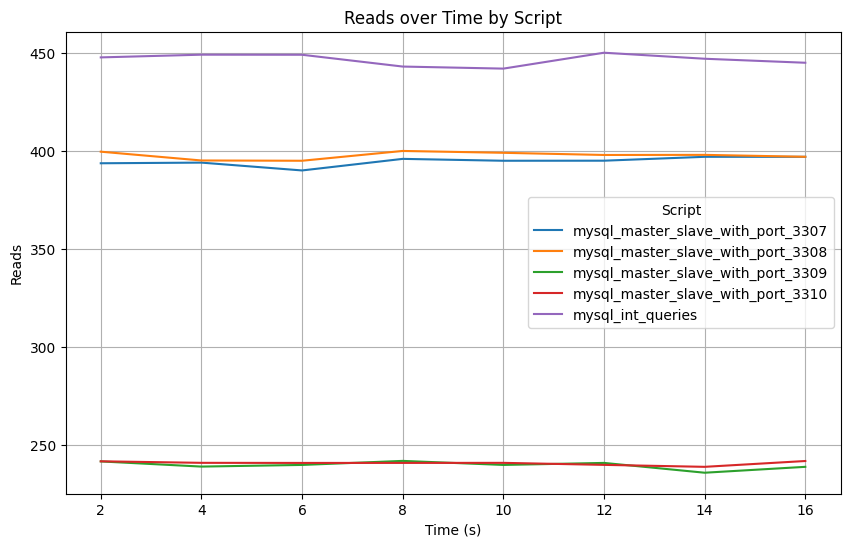
\includegraphics[width=\textwidth]{PNGs/Script/Replication/replication-vs-no/Reads}
    \label{replication-vs-no-reads}
  \end{subfigure}
  \hfill
  \begin{subfigure}[t]{0.48\textwidth}
    \centering
    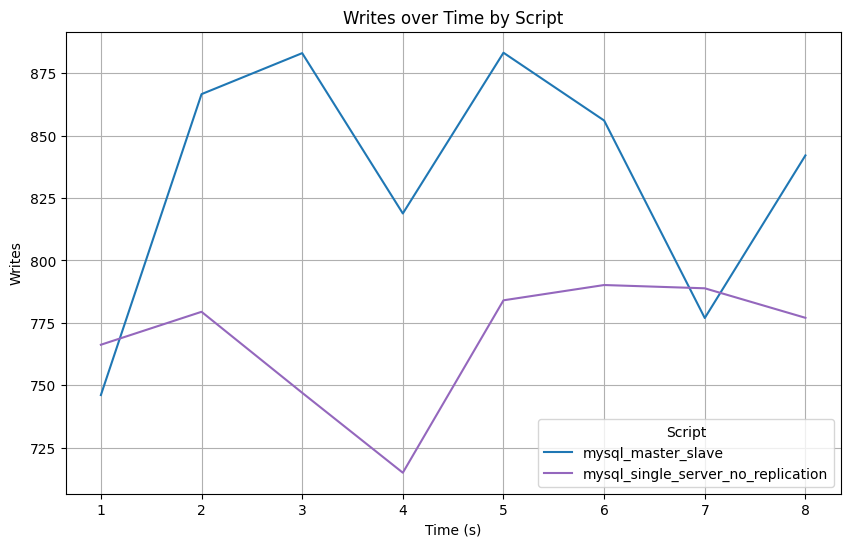
\includegraphics[width=\textwidth]{PNGs/Script/Replication/replication-vs-no/Writes}
    \label{replication-vs-no-writes}
  \end{subfigure}
  \vspace{-20pt}
  \caption[Replikation: Metrikvergleich]{Vergleich zwischen dem Master-Replica-Ansatz und einem normalen MySQL-Server }
  \label{fig:replication-vs-no}
\end{figure}
\vspace{-20pt}

Wenn wir die Ergebnisse aus Abbildung \ref{fig:replication-vs-no} betrachten, dann fällt auf, dass
//TODO (Daniel)

Im zweiten Vergleich benutzen wir ausschließlich den Master-Replica-Ansatz.
Dafür vergleichen wir aber die unterschiedlichen Binlog-Formate, die wir aus \ref{lst:repl_change_format} kennen.
Um Variationen zu begrenzen, betrachten wir nur eine Replica pro Master.
Das ergibt sechs unterschiedliche Leseergebnisse, da wir pro Format zwei Ports abfragen.
In der Grafik \ref{fig:replication-format-change} können wir sehen, dass die Unterschiedliche kaum erkennbar sind bei verschiedenen Binlog-Formaten und Ports.
Bei den Lesegeschwindigkeiten fallen aber durchaus Unterschiede auf.
//TODO (Daniel)

\begin{figure}[H]
  \centering
  \begin{subfigure}[t]{0.48\textwidth}
    \centering
    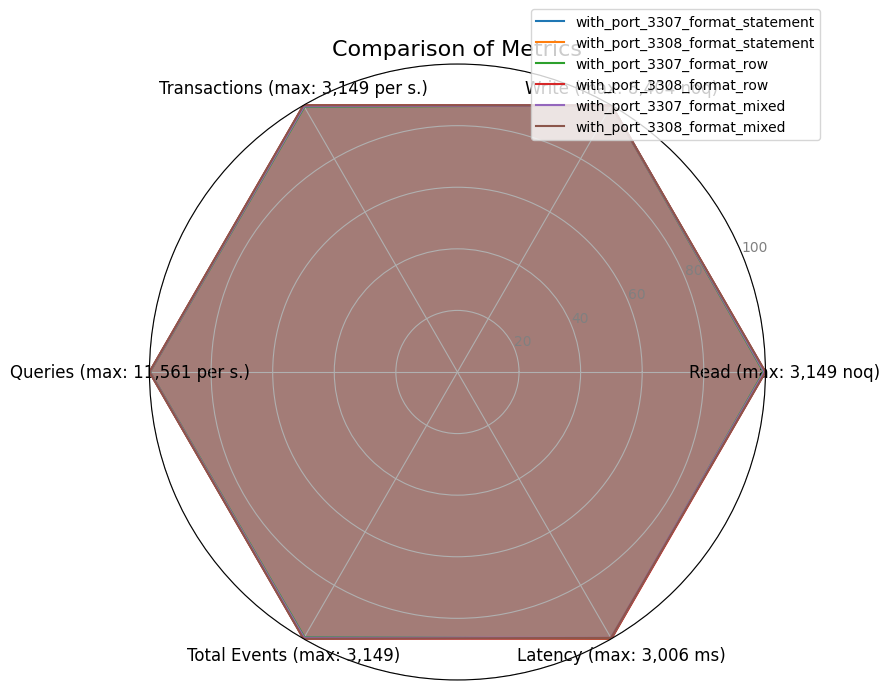
\includegraphics[width=\textwidth]{PNGs/Script/Replication/replication-format-change/statistics}
    \label{replication-format-change-statistics}
  \end{subfigure}
  \hfill
  \begin{subfigure}[t]{0.48\textwidth}
    \centering
    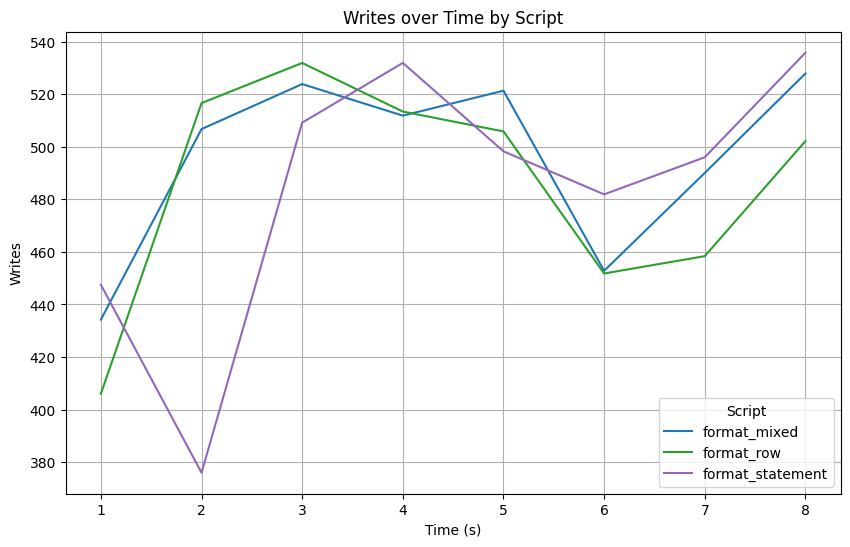
\includegraphics[width=\textwidth]{PNGs/Script/Replication/replication-format-change/Writes}
    \label{replication-format-change-writes}
  \end{subfigure}
  \vspace{-20pt}
  \caption[Replikation: Metrikvergleich]{Vergleich zwischen dem unterschiedlichen Binlog-Typen }
  \label{fig:replication-format-change}
\end{figure}
\vspace{-20pt}
